\documentclass[a4paper, colorlinks=false, 11pt, parskip=half,
               notitlepage, oneside, fleqn, pdftex]{scrartcl}

%%fakesection HEADER

%% ~ GRAPHICS / FIGURES
\usepackage{color}
\usepackage[pdftex,final]{graphicx}
\usepackage{fancyhdr}

%% ~ FONT / STYLE
\usepackage[UKenglish]{babel}
\usepackage[utf8]{inputenc}
\usepackage{lmodern}
\usepackage[T1]{fontenc}
\usepackage{verbatim}
\usepackage{upquote}
\usepackage[autostyle]{csquotes}
\usepackage{xspace}
\usepackage{natbib}
\usepackage[normalem]{ulem}

%% ~ PAGE LAYOUT
\usepackage[includeheadfoot, lmargin=3cm, rmargin=2cm,vmargin=2cm]{geometry}

%% ~ MATH RELATED
\usepackage{amssymb, amsmath, amsfonts}

%% ~ REFERENCING
\usepackage{lastpage}

%% ~ HYPERREF - SHOULD BE THE LAST PACKAGE LOADED
\usepackage[pdftex,final]{hyperref}

\frenchspacing

%% ~ CAPTIONS AND COLOURS
\definecolor{myblue}{rgb}{0,0,.8} % {0,0,.8}

\setlength\mathindent{0.5cm}
\renewcommand\baselinestretch{1.1}     % bigger line-spacing (everywhere)

%% ~ HEADER
\pagestyle{fancy}
\fancyhead{}  % clear all fields
\fancyfoot{}  % clear all fields
\renewcommand{\headrulewidth}{0pt}
\renewcommand{\footrulewidth}{0pt}
\fancyfoot[C]{\thepage/\pageref*{LastPage}}
% \fancyfoot[LE, LO]{}

%% ~ PDF-SETUP
\hypersetup{colorlinks=true, allcolors=myblue, breaklinks=true}

%% URL
\urlstyle{same}

\newcommand{\mr}[1]{\mathrm{#1}}



%%fakesection DOCUMENT
\begin{document}
\thispagestyle{empty}

\begin{centering}
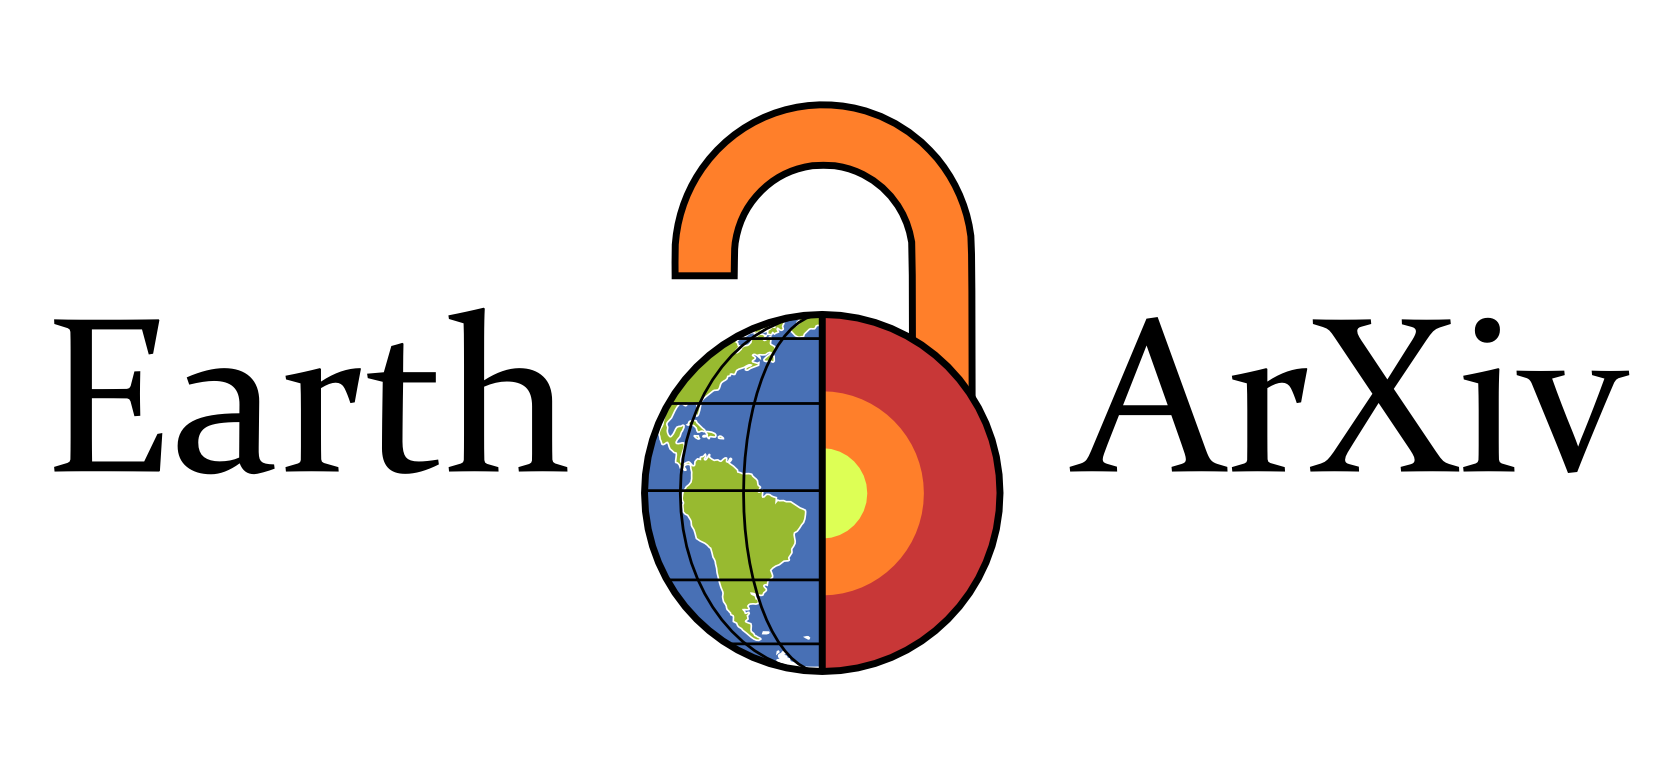
\includegraphics{ealogo.png}\\
\end{centering}

\bigskip

\textbf{\LARGE dageo: Data Assimilation in Geosciences}\\

\bigskip

\begin{itemize}
  \item \textbf{Dieter Werthmüller}$^{1, 2}$,
  \href{https://orcid.org/0000-0002-8575-2484}{0000-0002-8575-2484}
  \item \textbf{Gabriel Serrao Seabra}$^{1, 3}$,
  \href{https://orcid.org/0009-0002-0558-8117}{0009-0002-0558-8117}
  \item \textbf{Femke C. Vossepoel}$^{1}$,
  \href{https://orcid.org/0000-0002-3391-6651}{0000-0002-3391-6651}
\end{itemize}

{\small
  1: TU Delft, NL; 2: ETH Zurich, CH; 3: Petroleo Brasileiro S.A. (Petrobras), BR
}


\bigskip

{\Large
\textbf{Peer review status:}

This is a non-peer-reviewed preprint submitted to EarthArXiv.
}

\bigskip

This manuscript was submitted to the \emph{Journal of Open-Source Software}
(JOSS, \href{https://joss.theoj.org}{joss.theoj.org}) on 2025-03-06. It was
rejected on a preliminary scope query on 2025-04-02, on the ground that the
submission was deemed \emph{«too small in terms of substantial scholarly effort
to fit JOSS guidelines»}. See the pre-review issue on
\href{https://github.com/openjournals/joss-reviews/issues/7879}{github.com/openjournals/joss-reviews/issues/7879}.

We publish it here on EarthArXiv to make it nevertheless available to the
community. We might consider re-submission to JOSS at a later stage, once more
functionality is added to \texttt{dageo}.

\vfill

\texttt{dageo} (at \texttt{v1.1.1} at the time of this pre-print):
\begin{itemize}
  \item Repository:
    \href{https://github.com/tuda-geo/dageo}{github.com/tuda-geo/dageo}
  \item Zenodo:
    \href{https://doi.org/10.5281/zenodo.14264408}{doi.org/10.5281/zenodo.14264408}
  \item Documentation:
    \href{https://tuda-geo.github.io/dageo}{tuda-geo.github.io/dageo}
\end{itemize}

\newpage
\addtocounter{page}{-1}

\textbf{\LARGE dageo: Data Assimilation in Geosciences}\\

\textbf{\large
  Dieter Werthmüller$^{1, 2}$,
  Gabriel Serrao Seabra$^{1, 3}$,
  Femke C. Vossepoel$^{1}$
}

{\small
  1: TU Delft, NL; 2: ETH Zurich, CH; 3: Petroleo Brasileiro S.A. (Petrobras), BR
}



\section*{Summary}

Data Assimilation combines computer models with real-world measurements to
improve estimates and forecasts of dynamical systems such as oceans,
atmosphere, and subsurface reservoirs. The Python package \texttt{dageo} is a
tool to apply data assimilation in geoscience applications. Currently, it
encompasses the Ensemble Smoother with Multiple Data Assimilation (ESMDA)
method and provides tools for reservoir engineering applications. The package
includes localization to help with relatively small ensembles, Gaussian random
field generation for generating heterogeneous parameter fields, and integration
capabilities with external simulators.

An additional feature of \texttt{dageo} is a two-dimensional single-phase
reservoir simulator that models pressure changes over time and well behavior
for both injection and production scenarios. This simulator is particularly
useful for educational purposes, providing a practical platform for students
and researchers to learn and experiment with data assimilation concepts and
techniques. The software features an online documentation, with examples that
guide users through learning ESMDA concepts, testing new ideas, and applying
methods to real-world problems.

\section*{ESMDA}

Ensemble Smoother with Multiple Data Assimilation (ESMDA, \cite{esmda}) is the
first data assimilation method implemented in \texttt{dageo}. However,
\texttt{dageo} is general enough so that other data assimilation methods can
and will be added easily at a later stage. While ESMDA is theoretically
straightforward, practical implementation requires careful handling of matrix
operations, ensemble management, and ensuring numerical stability. The
algorithm works by iteratively updating an ensemble of model parameters to
match observed data following

\begin{equation}
  z_j^a = z_j^f + C_\mr{ZD}^f \left(C_\mr{DD}^f + \alpha C_\mr{D}
          \right)^{-1}\left(d_{\mr{uc},j} - d_j^f \right) \ ,
\end{equation}

where $z^a$ represents the updated (analysis) parameters, $z^f$ the prior
(forecast) parameters, and the $C$ terms represent various covariance matrices
for the data and the model parameters (subscripts D and Z, respectively). The
ESMDA coefficient (or inflation factor) is denoted by $\alpha$, the predicted
data vector, which is obtained by applying the observation operator to the
model output, is $d^f$ and $d_{\mr{uc}}$ represents the perturbed observations
\citep{burgers} for the j-th ensemble member, generated by adding random noise
to the original observations for each iteration, as proposed in the original
ESMDA method. Note that we assume to have an identity observation operator that
translates the model state to the equivalent of the observations, so it is
omitted in the equation (for more details in this regard see \cite{evensen}).
The equation is evaluated for $i$ steps, where $i$ is typically a low number
between 4 to 10. The $\alpha$ can change in each step, as long as $\sum_i
\alpha_i^{-1} = 1$. Common are either constant values or series of
decreasing values. Note that while this explanation describes the parameter
estimation problem, it could also be used to estimate the state estimation or
both. The algorithm's implementation in \texttt{dageo} includes optimizations
for efficient computation of the covariance matrix and allows to easily
parallelize the forward model.

\section*{Key Features and Applications}

Existing implementations often lack documentation and informative examples,
creating barriers for unexperienced users of data assimilation methods. These
challenges are addressed in \texttt{dageo} through several key innovations: it
provides a robust, tested ESMDA implementation alongside a built-in, simple
reservoir simulator, while offering and showcasing in the gallery, as a key
feature, integration capabilities with external simulators. The gallery
contains an example of this integration with the \emph{open Delft Advanced
Research Terra Simulator} \texttt{open-DARTS} \citep{opendarts}, a
state-of-the-art, open-source reservoir simulation framework developed at TU
Delft. It demonstrates how \texttt{dageo} can be used with industry-standard
simulators while maintaining its user-friendly interface. The code itself is
light, building upon NumPy arrays \citep{NumPy} and sparse matrices provided by
SciPy \citep{SciPy}, as only dependencies.

While other ESMDA implementations exist, e.g., \texttt{pyesmda}
\citep{pyesmda}, \texttt{dageo} distinguishes itself through comprehensive
documentation and examples, the integration of a simple but practical reservoir
simulator, the implementation of advanced features like localization techniques
for parameter updates, Gaussian random field generation for realistic
permeability modeling, and a focus on ease of use, making it suitable for
educational applications. This makes \texttt{dageo} a unique and valuable tool
for both research and teaching. The software has been used in several research
projects, including reservoir characterization studies at TU Delft, integration
with the open-DARTS simulator for geothermal applications, and educational
workshops on data assimilation techniques \citep[e.g.,][]{saifullin,seabra}.
These applications highlight the software's versatility and its ability to
address a wide range of challenges in reservoir engineering and geoscience.

\section*{Acknowledgements}

This work was supported by the \href{https://www.delphi-consortium.com}{Delphi
Consortium}. The authors thank Dr.~D.V. Voskov for his insights on implementing
a reservoir simulation.


\begin{thebibliography}{}
\itemsep0pt

\bibitem[Burgers et~al., 1998]{burgers}
Burgers, G., P.~J. van Leeuwen, and G. Evensen,  1998, Analysis scheme in the
  ensemble {K}alman filter: Monthly Weather Review, {\bfseries 126}, 1719 --
  1724; doi:
  \href{https://doi.org/10.1175/1520-0493(1998)126<1719:ASITEK>2.0.CO;2}{10.1175/1520-0493(1998)126<1719:ASITEK>2.0.CO;2}.

\bibitem[Collet, 2022]{pyesmda}
Collet, A.,  2022, {pyESMDA - Python Ensemble Smoother with Multiple Data
  Assimilation}; doi:
  \href{https://doi.org/10.5281/zenodo.7425669}{10.5281/zenodo.7425669}.

\bibitem[Emerick and Reynolds, 2013]{esmda}
Emerick, A.~A., and A.~C. Reynolds,  2013, Ensemble smoother with multiple data
  assimilation: Computers \& Geosciences, {\bfseries 55}, 3--15; doi:
  \href{https://doi.org/10.1016/j.cageo.2012.03.011}{10.1016/j.cageo.2012.03.011}.

\bibitem[Evensen et~al., 2022]{evensen}
Evensen, G., F.~C. Vossepoel, and P.~J. van Leeuwen,  2022, Data assimilation
  fundamentals: Springer.

\bibitem[Harris et~al., 2020]{NumPy}
Harris, C.~R., K.~J. Millman, S.~J. van~der Walt, R. Gommers, P. Virtanen, D.
  Cournapeau, E. Wieser, J. Taylor, S. Berg, N.~J. Smith, R. Kern, M. Picus, S.
  Hoyer, M.~H. van Kerkwijk, M. Brett, A. Haldane, J.~F. del R{\'{i}}o, M.
  Wiebe, P. Peterson, P. G{\'{e}}rard-Marchant, K. Sheppard, T. Reddy, W.
  Weckesser, H. Abbasi, C. Gohlke, and T.~E. Oliphant,  2020, Array programming
  with {NumPy}: Nature, {\bfseries 585}, 357--362; doi:
  \href{https://doi.org/10.1038/s41586-020-2649-2}{10.1038/s41586-020-2649-2}.

\bibitem[Saifullin et~al., 2024]{saifullin}
Saifullin, I., G.~S. Seabra, A. Pluymakers, F.~C. Vossepoel, and D. Voskov,
  2024, Integrating geomechanical proxy models with data assimilation for
  energy transition applications: Geomechanics for Energy and the Environment,
  {\bfseries 40}, 100618; doi:
  \href{https://doi.org/10.1016/j.gete.2024.100618}{10.1016/j.gete.2024.100618}.

\bibitem[Seabra et~al., 2024]{seabra}
Seabra, G.~S., N.~T. Mücke, V.~L.~S. Silva, D. Voskov, and F.~C. Vossepoel,
  2024, Ai enhanced data assimilation and uncertainty quantification applied to
  geological carbon storage: International Journal of Greenhouse Gas Control,
  {\bfseries 136}, 104190; doi:
  \href{https://doi.org/10.1016/j.ijggc.2024.104190}{10.1016/j.ijggc.2024.104190}.

\bibitem[Virtanen et~al., 2020]{SciPy}
Virtanen, P., R. Gommers, T.~E. Oliphant, M. Haberland, T. Reddy, D.
  Cournapeau, E. Burovski, P. Peterson, W. Weckesser, J. Bright, S.~J. {van der
  Walt}, M. Brett, J. Wilson, K.~J. Millman, N. Mayorov, A.~R.~J. Nelson, E.
  Jones, R. Kern, E. Larson, C.~J. Carey, {\.I}. Polat, Y. Feng, E.~W. Moore,
  J. {VanderPlas}, D. Laxalde, J. Perktold, R. Cimrman, I. Henriksen, E.~A.
  Quintero, C.~R. Harris, A.~M. Archibald, A.~H. Ribeiro, F. Pedregosa, P. {van
  Mulbregt}, and {SciPy 1.0 Contributors},  2020, {{SciPy} 1.0: Fundamental
  Algorithms for Scientific Computing in Python}: Nature Methods, {\bfseries
  17}, 261--272; doi:
  \href{https://doi.org/10.1038/s41592-019-0686-2}{10.1038/s41592-019-0686-2}.

\bibitem[Voskov et~al., 2024]{opendarts}
Voskov, D., I. Saifullin, A. Novikov, M. Wapperom, L. Orozco, G.~S. Seabra, Y.
  Chen, M. Khait, X. Lyu, X. Tian, S. de~Hoop, and A. Palha,  2024, open
  {D}elft {A}dvanced {R}esearch {T}erra {S}imulator (open-{DARTS}): Journal of
  Open Source Software, {\bfseries 9}, 6737; doi:
  \href{https://doi.org/10.21105/joss.06737}{10.21105/joss.06737}.

\end{thebibliography}

\end{document}
